\documentclass[twoside]{book}

% Packages required by doxygen
\usepackage{fixltx2e}
\usepackage{calc}
\usepackage{doxygen}
\usepackage[export]{adjustbox} % also loads graphicx
\usepackage{graphicx}
\usepackage[utf8]{inputenc}
\usepackage{makeidx}
\usepackage{multicol}
\usepackage{multirow}
\PassOptionsToPackage{warn}{textcomp}
\usepackage{textcomp}
\usepackage[nointegrals]{wasysym}
\usepackage[table]{xcolor}

% Font selection
\usepackage[T1]{fontenc}
\usepackage[scaled=.90]{helvet}
\usepackage{courier}
\usepackage{amssymb}
\usepackage{sectsty}
\renewcommand{\familydefault}{\sfdefault}
\allsectionsfont{%
  \fontseries{bc}\selectfont%
  \color{darkgray}%
}
\renewcommand{\DoxyLabelFont}{%
  \fontseries{bc}\selectfont%
  \color{darkgray}%
}
\newcommand{\+}{\discretionary{\mbox{\scriptsize$\hookleftarrow$}}{}{}}

% Page & text layout
\usepackage{geometry}
\geometry{%
  a4paper,%
  top=2.5cm,%
  bottom=2.5cm,%
  left=2.5cm,%
  right=2.5cm%
}
\tolerance=750
\hfuzz=15pt
\hbadness=750
\setlength{\emergencystretch}{15pt}
\setlength{\parindent}{0cm}
\setlength{\parskip}{3ex plus 2ex minus 2ex}
\makeatletter
\renewcommand{\paragraph}{%
  \@startsection{paragraph}{4}{0ex}{-1.0ex}{1.0ex}{%
    \normalfont\normalsize\bfseries\SS@parafont%
  }%
}
\renewcommand{\subparagraph}{%
  \@startsection{subparagraph}{5}{0ex}{-1.0ex}{1.0ex}{%
    \normalfont\normalsize\bfseries\SS@subparafont%
  }%
}
\makeatother

% Headers & footers
\usepackage{fancyhdr}
\pagestyle{fancyplain}
\fancyhead[LE]{\fancyplain{}{\bfseries\thepage}}
\fancyhead[CE]{\fancyplain{}{}}
\fancyhead[RE]{\fancyplain{}{\bfseries\leftmark}}
\fancyhead[LO]{\fancyplain{}{\bfseries\rightmark}}
\fancyhead[CO]{\fancyplain{}{}}
\fancyhead[RO]{\fancyplain{}{\bfseries\thepage}}
\fancyfoot[LE]{\fancyplain{}{}}
\fancyfoot[CE]{\fancyplain{}{}}
\fancyfoot[RE]{\fancyplain{}{\bfseries\scriptsize Generated by Doxygen }}
\fancyfoot[LO]{\fancyplain{}{\bfseries\scriptsize Generated by Doxygen }}
\fancyfoot[CO]{\fancyplain{}{}}
\fancyfoot[RO]{\fancyplain{}{}}
\renewcommand{\footrulewidth}{0.4pt}
\renewcommand{\chaptermark}[1]{%
  \markboth{#1}{}%
}
\renewcommand{\sectionmark}[1]{%
  \markright{\thesection\ #1}%
}

% Indices & bibliography
\usepackage{natbib}
\usepackage[titles]{tocloft}
\setcounter{tocdepth}{3}
\setcounter{secnumdepth}{5}
\makeindex

% Hyperlinks (required, but should be loaded last)
\usepackage{ifpdf}
\ifpdf
  \usepackage[pdftex,pagebackref=true]{hyperref}
\else
  \usepackage[ps2pdf,pagebackref=true]{hyperref}
\fi
\hypersetup{%
  colorlinks=true,%
  linkcolor=blue,%
  citecolor=blue,%
  unicode%
}

% Custom commands
\newcommand{\clearemptydoublepage}{%
  \newpage{\pagestyle{empty}\cleardoublepage}%
}

\usepackage{caption}
\captionsetup{labelsep=space,justification=centering,font={bf},singlelinecheck=off,skip=4pt,position=top}

%===== C O N T E N T S =====

\begin{document}

% Titlepage & ToC
\hypersetup{pageanchor=false,
             bookmarksnumbered=true,
             pdfencoding=unicode
            }
\pagenumbering{roman}
\begin{titlepage}
\vspace*{7cm}
\begin{center}%
{\Large Electric Tiger D\+AQ \\[1ex]\large 0.\+1 }\\
\vspace*{1cm}
{\large Generated by Doxygen 1.8.11}\\
\end{center}
\end{titlepage}
\clearemptydoublepage
\tableofcontents
\clearemptydoublepage
\pagenumbering{arabic}
\hypersetup{pageanchor=true}

%--- Begin generated contents ---
\chapter{Hierarchical Index}
\section{Class Hierarchy}
This inheritance list is sorted roughly, but not completely, alphabetically\+:\begin{DoxyCompactList}
\item \contentsline{section}{Abstract\+Socket\+Communicator}{\pageref{class_abstract_socket_communicator}}{}
\begin{DoxyCompactList}
\item \contentsline{section}{Arduino}{\pageref{class_arduino}}{}
\item \contentsline{section}{Network\+Analyzer}{\pageref{class_network_analyzer}}{}
\end{DoxyCompactList}
\item Q\+Chart\+View\begin{DoxyCompactList}
\item \contentsline{section}{Spectrum\+Analyzer}{\pageref{class_spectrum_analyzer}}{}
\end{DoxyCompactList}
\item Q\+Dock\+Widget\begin{DoxyCompactList}
\item \contentsline{section}{Frequency\+Controls}{\pageref{class_frequency_controls}}{}
\item \contentsline{section}{Power\+Controls}{\pageref{class_power_controls}}{}
\end{DoxyCompactList}
\item Q\+Main\+Window\begin{DoxyCompactList}
\item \contentsline{section}{Main\+Window}{\pageref{class_main_window}}{}
\end{DoxyCompactList}
\item Q\+Menu\begin{DoxyCompactList}
\item \contentsline{section}{Right\+Click\+Menu}{\pageref{class_right_click_menu}}{}
\end{DoxyCompactList}
\item Q\+Object\begin{DoxyCompactList}
\item \contentsline{section}{Q\+Socket\+Comm}{\pageref{class_q_socket_comm}}{}
\end{DoxyCompactList}
\item \contentsline{section}{Signal\+Generator}{\pageref{class_signal_generator}}{}
\item \contentsline{section}{Socket\+Comm}{\pageref{class_socket_comm}}{}
\item \contentsline{section}{Stepper\+Motor}{\pageref{class_stepper_motor}}{}
\item \contentsline{section}{Switch}{\pageref{class_switch}}{}
\item \contentsline{section}{Volts\+Tod\+Bm\+\_\+\+F\+F\+T\+Correction}{\pageref{struct_volts_tod_bm___f_f_t_correction}}{}
\end{DoxyCompactList}

\chapter{Class Index}
\section{Class List}
Here are the classes, structs, unions and interfaces with brief descriptions\+:\begin{DoxyCompactList}
\item\contentsline{section}{\hyperlink{class_abstract_socket_communicator}{Abstract\+Socket\+Communicator} }{\pageref{class_abstract_socket_communicator}}{}
\item\contentsline{section}{\hyperlink{class_arduino}{Arduino} \\*Object to send and receive commands from an \hyperlink{class_arduino}{Arduino} Uno (R3) }{\pageref{class_arduino}}{}
\item\contentsline{section}{\hyperlink{class_frequency_controls}{Frequency\+Controls} }{\pageref{class_frequency_controls}}{}
\item\contentsline{section}{\hyperlink{class_main_window}{Main\+Window} }{\pageref{class_main_window}}{}
\item\contentsline{section}{\hyperlink{class_network_analyzer}{Network\+Analyzer} \\*Object to communicate with the H\+P8757 C Network Analyzer }{\pageref{class_network_analyzer}}{}
\item\contentsline{section}{\hyperlink{class_power_controls}{Power\+Controls} }{\pageref{class_power_controls}}{}
\item\contentsline{section}{\hyperlink{class_q_socket_comm}{Q\+Socket\+Comm} }{\pageref{class_q_socket_comm}}{}
\item\contentsline{section}{\hyperlink{class_right_click_menu}{Right\+Click\+Menu} }{\pageref{class_right_click_menu}}{}
\item\contentsline{section}{\hyperlink{class_signal_generator}{Signal\+Generator} }{\pageref{class_signal_generator}}{}
\item\contentsline{section}{\hyperlink{class_socket_comm}{Socket\+Comm} }{\pageref{class_socket_comm}}{}
\item\contentsline{section}{\hyperlink{class_spectrum_analyzer}{Spectrum\+Analyzer} }{\pageref{class_spectrum_analyzer}}{}
\item\contentsline{section}{\hyperlink{class_stepper_motor}{Stepper\+Motor} }{\pageref{class_stepper_motor}}{}
\item\contentsline{section}{\hyperlink{class_switch}{Switch} }{\pageref{class_switch}}{}
\item\contentsline{section}{\hyperlink{struct_volts_tod_bm___f_f_t_correction}{Volts\+Tod\+Bm\+\_\+\+F\+F\+T\+Correction} }{\pageref{struct_volts_tod_bm___f_f_t_correction}}{}
\end{DoxyCompactList}

\chapter{Class Documentation}
\hypertarget{class_abstract_socket_communicator}{}\section{Abstract\+Socket\+Communicator Class Reference}
\label{class_abstract_socket_communicator}\index{Abstract\+Socket\+Communicator@{Abstract\+Socket\+Communicator}}


Inheritance diagram for Abstract\+Socket\+Communicator\+:
\nopagebreak
\begin{figure}[H]
\begin{center}
\leavevmode
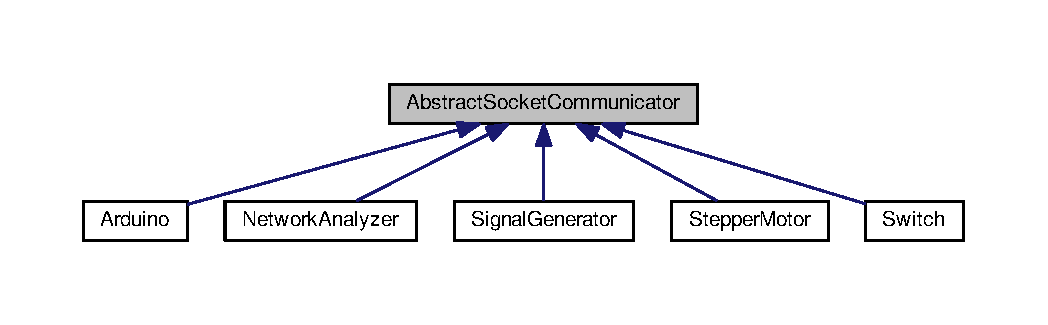
\includegraphics[width=350pt]{class_abstract_socket_communicator__inherit__graph}
\end{center}
\end{figure}


Collaboration diagram for Abstract\+Socket\+Communicator\+:\nopagebreak
\begin{figure}[H]
\begin{center}
\leavevmode
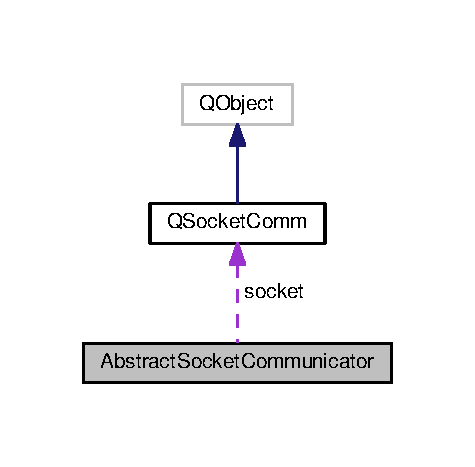
\includegraphics[width=228pt]{class_abstract_socket_communicator__coll__graph}
\end{center}
\end{figure}
\subsection*{Public Member Functions}
\begin{DoxyCompactItemize}
\item 
{\bfseries Abstract\+Socket\+Communicator} (std\+::string ip\+\_\+addr, uint port\+\_\+number)\hypertarget{class_abstract_socket_communicator_a94b6e0b544fadba42bd3a5c6f4a549fd}{}\label{class_abstract_socket_communicator_a94b6e0b544fadba42bd3a5c6f4a549fd}

\item 
{\bfseries Abstract\+Socket\+Communicator} (const \hyperlink{struct_t_c_p_socket_param}{T\+C\+P\+Socket\+Param} socket\+\_\+param)\hypertarget{class_abstract_socket_communicator_a0d5d09d52f50e951ee7d5710b06a7a9d}{}\label{class_abstract_socket_communicator_a0d5d09d52f50e951ee7d5710b06a7a9d}

\item 
\hyperlink{class_abstract_socket_communicator}{Abstract\+Socket\+Communicator} \& {\bfseries operator=} (const \hyperlink{class_abstract_socket_communicator}{Abstract\+Socket\+Communicator} \&)=delete\hypertarget{class_abstract_socket_communicator_a7ee57a3af5927ac08f515055dbcdc829}{}\label{class_abstract_socket_communicator_a7ee57a3af5927ac08f515055dbcdc829}

\end{DoxyCompactItemize}
\subsection*{Protected Attributes}
\begin{DoxyCompactItemize}
\item 
\hyperlink{class_q_socket_comm}{Q\+Socket\+Comm} $\ast$ {\bfseries socket}\hypertarget{class_abstract_socket_communicator_a7e69037572c26cf596bd117490f9d6c1}{}\label{class_abstract_socket_communicator_a7e69037572c26cf596bd117490f9d6c1}

\end{DoxyCompactItemize}


The documentation for this class was generated from the following files\+:\begin{DoxyCompactItemize}
\item 
/home/bephillips2/\+Qt-\/\+Projects/\+Electric\+\_\+\+Tiger\+\_\+\+D\+A\+Q/\+Socket\+Communicators/\+Abstract\+Socket\+Communicator/abstractsocketcommunictor.\+h\item 
/home/bephillips2/\+Qt-\/\+Projects/\+Electric\+\_\+\+Tiger\+\_\+\+D\+A\+Q/\+Socket\+Communicators/\+Abstract\+Socket\+Communicator/abstractsocketcommunictor.\+cpp\end{DoxyCompactItemize}

\hypertarget{class_arduino}{\section{Arduino Class Reference}
\label{class_arduino}\index{Arduino@{Arduino}}
}


Object to send and receive commands from an \hyperlink{class_arduino}{Arduino} Uno (R3)  




{\ttfamily \#include $<$arduino.\+h$>$}



Inheritance diagram for Arduino\+:\nopagebreak
\begin{figure}[H]
\begin{center}
\leavevmode
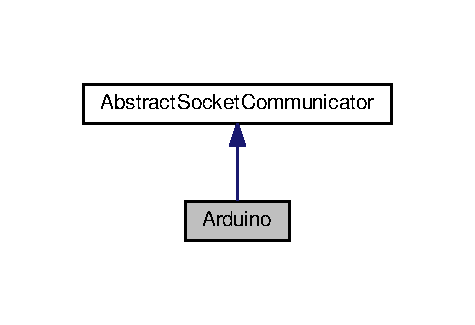
\includegraphics[width=228pt]{class_arduino__inherit__graph}
\end{center}
\end{figure}


Collaboration diagram for Arduino\+:\nopagebreak
\begin{figure}[H]
\begin{center}
\leavevmode
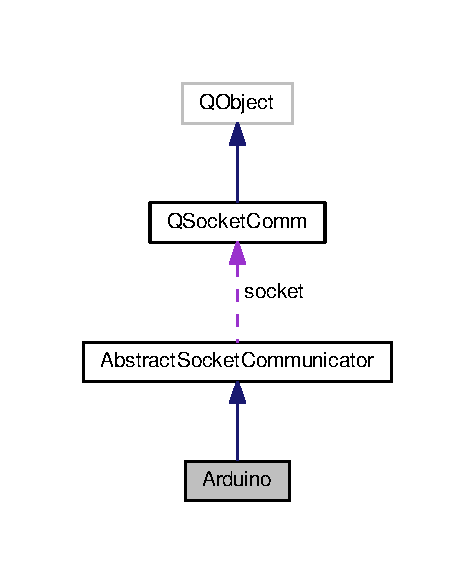
\includegraphics[width=228pt]{class_arduino__coll__graph}
\end{center}
\end{figure}
\subsection*{Public Member Functions}
\begin{DoxyCompactItemize}
\item 
\hypertarget{class_arduino_a92c95a8b8c1022d0145da24d53a1db7b}{{\bfseries Arduino} (std\+::string ip\+\_\+addr, uint port\+\_\+number)}\label{class_arduino_a92c95a8b8c1022d0145da24d53a1db7b}

\item 
\hypertarget{class_arduino_a73d294f82c38557d1872cadd372c0b8b}{\hyperlink{class_arduino}{Arduino} \& {\bfseries operator=} (const \hyperlink{class_arduino}{Arduino} \&)=delete}\label{class_arduino_a73d294f82c38557d1872cadd372c0b8b}

\item 
double \hyperlink{class_arduino_a0ae462174c61881ccd5f78af5130eceb}{Get\+Cavity\+Length} ()
\begin{DoxyCompactList}\small\item\em Get the current cavity length from the \hyperlink{class_arduino}{Arduino}. \end{DoxyCompactList}\end{DoxyCompactItemize}
\subsection*{Additional Inherited Members}


\subsection{Detailed Description}
Object to send and receive commands from an \hyperlink{class_arduino}{Arduino} Uno (R3) 

\hyperlink{class_arduino}{Arduino} is expected to be equipped with an Ethernet Shield and string potentiometer. 

\subsection{Member Function Documentation}
\hypertarget{class_arduino_a0ae462174c61881ccd5f78af5130eceb}{\index{Arduino@{Arduino}!Get\+Cavity\+Length@{Get\+Cavity\+Length}}
\index{Get\+Cavity\+Length@{Get\+Cavity\+Length}!Arduino@{Arduino}}
\subsubsection[{Get\+Cavity\+Length}]{\setlength{\rightskip}{0pt plus 5cm}double Arduino\+::\+Get\+Cavity\+Length (
\begin{DoxyParamCaption}
{}
\end{DoxyParamCaption}
)}}\label{class_arduino_a0ae462174c61881ccd5f78af5130eceb}


Get the current cavity length from the \hyperlink{class_arduino}{Arduino}. 

This function will poll the \hyperlink{class_arduino}{Arduino} until a non-\/empty string is returned, guaranteeing that the return value will be valid.

Note that this does not elminate the problem of getting 'doubled' responses, e.\+g. \char`\"{}7.\+5\textbackslash{}r\textbackslash{}n7.\+5\char`\"{}

\begin{DoxyReturn}{Returns}
Current length of the cavity, in inches 
\end{DoxyReturn}


The documentation for this class was generated from the following files\+:\begin{DoxyCompactItemize}
\item 
/home/admx/\+Qt-\/\+Projects/\+Electric\+\_\+\+Tiger\+\_\+\+D\+A\+Q/\+Socket\+Communicators/\+Arduino/arduino.\+h\item 
/home/admx/\+Qt-\/\+Projects/\+Electric\+\_\+\+Tiger\+\_\+\+D\+A\+Q/\+Socket\+Communicators/\+Arduino/arduino.\+cpp\end{DoxyCompactItemize}

\hypertarget{class_frequency_controls}{}\section{Frequency\+Controls Class Reference}
\label{class_frequency_controls}\index{Frequency\+Controls@{Frequency\+Controls}}


Inheritance diagram for Frequency\+Controls\+:
\nopagebreak
\begin{figure}[H]
\begin{center}
\leavevmode
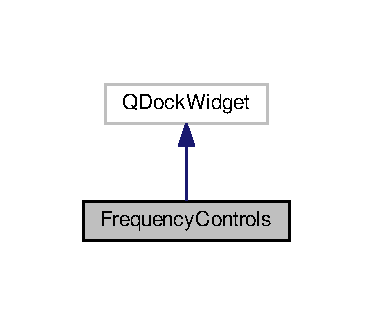
\includegraphics[width=179pt]{class_frequency_controls__inherit__graph}
\end{center}
\end{figure}


Collaboration diagram for Frequency\+Controls\+:
\nopagebreak
\begin{figure}[H]
\begin{center}
\leavevmode
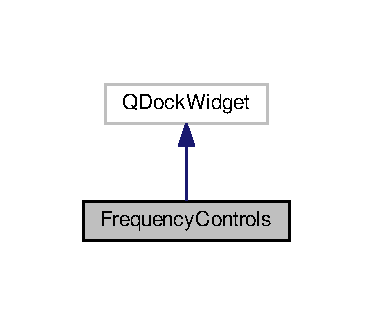
\includegraphics[width=179pt]{class_frequency_controls__coll__graph}
\end{center}
\end{figure}
\subsection*{Public Slots}
\begin{DoxyCompactItemize}
\item 
void {\bfseries Set\+Freq\+Span} (int span)\hypertarget{class_frequency_controls_a88109da989b014a69677728e96bb6a8a}{}\label{class_frequency_controls_a88109da989b014a69677728e96bb6a8a}

\item 
void {\bfseries Set\+Min\+Max} (std\+::pair$<$ int, int $>$ vals)\hypertarget{class_frequency_controls_acf2eee8710eac492be4004217fbbafd1}{}\label{class_frequency_controls_acf2eee8710eac492be4004217fbbafd1}

\end{DoxyCompactItemize}
\subsection*{Signals}
\begin{DoxyCompactItemize}
\item 
void {\bfseries Min\+Set} (double min\+\_\+val)\hypertarget{class_frequency_controls_a3544c74823a7aaabc9a0779ae839eb7f}{}\label{class_frequency_controls_a3544c74823a7aaabc9a0779ae839eb7f}

\item 
void {\bfseries Max\+Set} (double max\+\_\+val)\hypertarget{class_frequency_controls_ad8606de91f4ec71aa8011f658da35a4e}{}\label{class_frequency_controls_ad8606de91f4ec71aa8011f658da35a4e}

\item 
void {\bfseries Unit\+Selected} (Q\+String units)\hypertarget{class_frequency_controls_a5b873965eb03064dbcf713d0c66126d0}{}\label{class_frequency_controls_a5b873965eb03064dbcf713d0c66126d0}

\item 
void {\bfseries Span\+Set} (int span\+\_\+val)\hypertarget{class_frequency_controls_aef534d12777d179c45b59a47c8c1b431}{}\label{class_frequency_controls_aef534d12777d179c45b59a47c8c1b431}

\item 
void {\bfseries Center\+Set} (int cent\+\_\+val)\hypertarget{class_frequency_controls_afd8a0e6ada7b9063e15d55c9c6b562cb}{}\label{class_frequency_controls_afd8a0e6ada7b9063e15d55c9c6b562cb}

\end{DoxyCompactItemize}
\subsection*{Public Member Functions}
\begin{DoxyCompactItemize}
\item 
{\bfseries Frequency\+Controls} (Q\+Widget $\ast$parent=0)\hypertarget{class_frequency_controls_a41928b0575667ca2677e824a0907285b}{}\label{class_frequency_controls_a41928b0575667ca2677e824a0907285b}

\end{DoxyCompactItemize}


The documentation for this class was generated from the following files\+:\begin{DoxyCompactItemize}
\item 
/home/bephillips2/\+Qt-\/\+Projects/\+Electric\+\_\+\+Tiger\+\_\+\+D\+A\+Q/\+Spectrum\+Analyzer/\+Graphic\+Objects/frequencycontrols.\+h\item 
/home/bephillips2/\+Qt-\/\+Projects/\+Electric\+\_\+\+Tiger\+\_\+\+D\+A\+Q/\+Spectrum\+Analyzer/\+Graphic\+Objects/frequencycontrols.\+cpp\end{DoxyCompactItemize}

\hypertarget{class_main_window}{}\section{Main\+Window Class Reference}
\label{class_main_window}\index{Main\+Window@{Main\+Window}}


Inheritance diagram for Main\+Window\+:\nopagebreak
\begin{figure}[H]
\begin{center}
\leavevmode
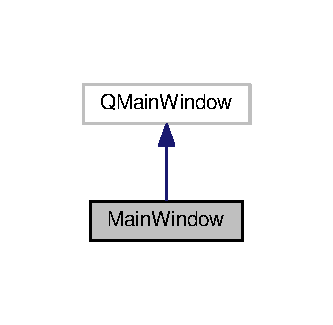
\includegraphics[width=160pt]{class_main_window__inherit__graph}
\end{center}
\end{figure}


Collaboration diagram for Main\+Window\+:\nopagebreak
\begin{figure}[H]
\begin{center}
\leavevmode
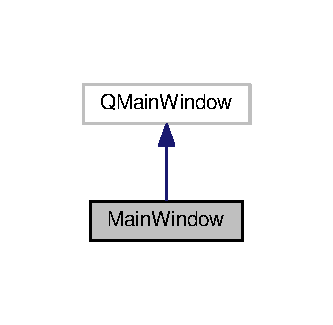
\includegraphics[width=160pt]{class_main_window__coll__graph}
\end{center}
\end{figure}
\subsection*{Public Member Functions}
\begin{DoxyCompactItemize}
\item 
{\bfseries Main\+Window} (Q\+Widget $\ast$parent=0)\hypertarget{class_main_window_a8b244be8b7b7db1b08de2a2acb9409db}{}\label{class_main_window_a8b244be8b7b7db1b08de2a2acb9409db}

\end{DoxyCompactItemize}


The documentation for this class was generated from the following files\+:\begin{DoxyCompactItemize}
\item 
/home/bephillips2/\+Qt-\/\+Projects/\+Electric\+\_\+\+Tiger\+\_\+\+D\+A\+Q/mainwindow.\+h\item 
/home/bephillips2/\+Qt-\/\+Projects/\+Electric\+\_\+\+Tiger\+\_\+\+D\+A\+Q/mainwindow.\+cpp\end{DoxyCompactItemize}

\hypertarget{class_network_analyzer}{\section{Network\+Analyzer Class Reference}
\label{class_network_analyzer}\index{Network\+Analyzer@{Network\+Analyzer}}
}


Object to communicate with the H\+P8757 C Network Analyzer.  




{\ttfamily \#include $<$network\+\_\+analyzer.\+h$>$}



Inheritance diagram for Network\+Analyzer\+:\nopagebreak
\begin{figure}[H]
\begin{center}
\leavevmode
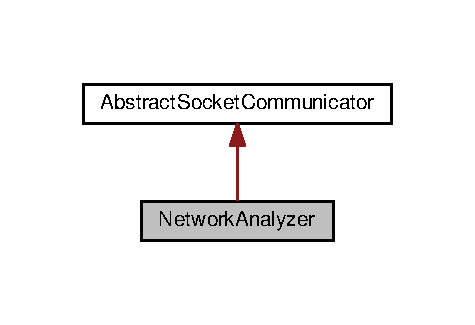
\includegraphics[width=228pt]{class_network_analyzer__inherit__graph}
\end{center}
\end{figure}


Collaboration diagram for Network\+Analyzer\+:\nopagebreak
\begin{figure}[H]
\begin{center}
\leavevmode
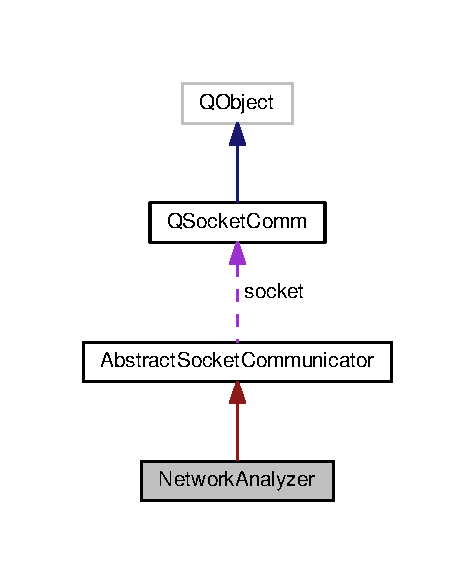
\includegraphics[width=228pt]{class_network_analyzer__coll__graph}
\end{center}
\end{figure}
\subsection*{Public Member Functions}
\begin{DoxyCompactItemize}
\item 
\hypertarget{class_network_analyzer_a1d8a2de50a5079e392e912e3bc25cbbb}{{\bfseries Network\+Analyzer} (std\+::string ip\+\_\+addr, uint port\+\_\+number, uint points, double span, double power)}\label{class_network_analyzer_a1d8a2de50a5079e392e912e3bc25cbbb}

\item 
\hypertarget{class_network_analyzer_a2785c012d28fb621e7218a9e471716e3}{\hyperlink{class_network_analyzer}{Network\+Analyzer} \& {\bfseries operator=} (const \hyperlink{class_network_analyzer}{Network\+Analyzer} \&)=delete}\label{class_network_analyzer_a2785c012d28fb621e7218a9e471716e3}

\item 
\hypertarget{class_network_analyzer_a667cf86a80639bb57c67061b7c9df210}{std\+::vector$<$ double $>$ {\bfseries Take\+Data\+Multiple} ()}\label{class_network_analyzer_a667cf86a80639bb57c67061b7c9df210}

\item 
std\+::vector$<$ double $>$ \hyperlink{class_network_analyzer_aa7ae9c649f4d7a5828e2d24ad8dee65d}{Take\+Data\+Single} ()
\begin{DoxyCompactList}\small\item\em Collect a single power spectrum from the Network Analyzer. \end{DoxyCompactList}\item 
\hypertarget{class_network_analyzer_a65864fe6142eadfd8e3e976e592e4bf0}{void {\bfseries Set\+Frequency\+Window} (double frequency, double frequency\+\_\+span)}\label{class_network_analyzer_a65864fe6142eadfd8e3e976e592e4bf0}

\item 
\hypertarget{class_network_analyzer_a5d986f4eb0ed10030ba02ef43b65ac30}{void {\bfseries Set\+Frequency\+Span} (double frequency\+\_\+span)}\label{class_network_analyzer_a5d986f4eb0ed10030ba02ef43b65ac30}

\item 
\hypertarget{class_network_analyzer_a6d4e76a043fd30788167c4c0e187ed00}{void \hyperlink{class_network_analyzer_a6d4e76a043fd30788167c4c0e187ed00}{Turn\+On\+R\+F\+Source} ()}\label{class_network_analyzer_a6d4e76a043fd30788167c4c0e187ed00}

\begin{DoxyCompactList}\small\item\em Turn the R\+F source on, at whatever power it was set to most recently. \end{DoxyCompactList}\item 
\hypertarget{class_network_analyzer_aeeb9823df08d7b602d524583fcc94c26}{void \hyperlink{class_network_analyzer_aeeb9823df08d7b602d524583fcc94c26}{Turn\+Off\+R\+F\+Source} ()}\label{class_network_analyzer_aeeb9823df08d7b602d524583fcc94c26}

\begin{DoxyCompactList}\small\item\em Turn the R\+F source off. \end{DoxyCompactList}\end{DoxyCompactItemize}
\subsection*{Additional Inherited Members}


\subsection{Detailed Description}
Object to communicate with the H\+P8757 C Network Analyzer. 

\subsection{Member Function Documentation}
\hypertarget{class_network_analyzer_aa7ae9c649f4d7a5828e2d24ad8dee65d}{\index{Network\+Analyzer@{Network\+Analyzer}!Take\+Data\+Single@{Take\+Data\+Single}}
\index{Take\+Data\+Single@{Take\+Data\+Single}!Network\+Analyzer@{Network\+Analyzer}}
\subsubsection[{Take\+Data\+Single}]{\setlength{\rightskip}{0pt plus 5cm}std\+::vector$<$ double $>$ Network\+Analyzer\+::\+Take\+Data\+Single (
\begin{DoxyParamCaption}
{}
\end{DoxyParamCaption}
)}}\label{class_network_analyzer_aa7ae9c649f4d7a5828e2d24ad8dee65d}


Collect a single power spectrum from the Network Analyzer. 

Settings will be whatever the Network Analyzer was set to when this function is called. \begin{DoxyReturn}{Returns}

\end{DoxyReturn}


The documentation for this class was generated from the following files\+:\begin{DoxyCompactItemize}
\item 
/home/admx/\+Qt-\/\+Projects/\+Electric\+\_\+\+Tiger\+\_\+\+D\+A\+Q/\+Socket\+Communicators/\+Network\+Analyzer/network\+\_\+analyzer.\+h\item 
/home/admx/\+Qt-\/\+Projects/\+Electric\+\_\+\+Tiger\+\_\+\+D\+A\+Q/\+Socket\+Communicators/\+Network\+Analyzer/network\+\_\+analyzer.\+cpp\end{DoxyCompactItemize}

\hypertarget{class_power_controls}{}\section{Power\+Controls Class Reference}
\label{class_power_controls}\index{Power\+Controls@{Power\+Controls}}


Inheritance diagram for Power\+Controls\+:\nopagebreak
\begin{figure}[H]
\begin{center}
\leavevmode
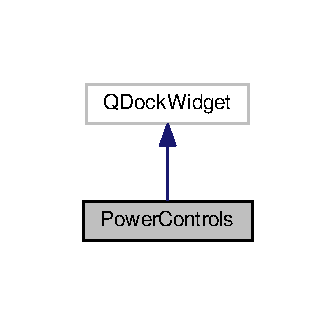
\includegraphics[width=161pt]{class_power_controls__inherit__graph}
\end{center}
\end{figure}


Collaboration diagram for Power\+Controls\+:\nopagebreak
\begin{figure}[H]
\begin{center}
\leavevmode
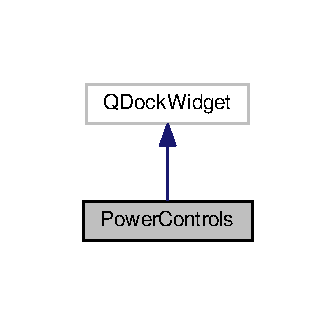
\includegraphics[width=161pt]{class_power_controls__coll__graph}
\end{center}
\end{figure}
\subsection*{Public Slots}
\begin{DoxyCompactItemize}
\item 
void {\bfseries Set\+Freq\+Span} (int span)\hypertarget{class_power_controls_a9bd193055b86e97e51d96912271fffe5}{}\label{class_power_controls_a9bd193055b86e97e51d96912271fffe5}

\item 
void {\bfseries Set\+Min\+Max} (std\+::pair$<$ int, int $>$ vals)\hypertarget{class_power_controls_afa8e34d9a376e9abc0839e3caafa6ab9}{}\label{class_power_controls_afa8e34d9a376e9abc0839e3caafa6ab9}

\end{DoxyCompactItemize}
\subsection*{Signals}
\begin{DoxyCompactItemize}
\item 
void {\bfseries Min\+Set} (double min\+\_\+val)\hypertarget{class_power_controls_ab9a1d9f89f194471d0e31f6dad01086a}{}\label{class_power_controls_ab9a1d9f89f194471d0e31f6dad01086a}

\item 
void {\bfseries Max\+Set} (double max\+\_\+val)\hypertarget{class_power_controls_aef88de9bf3ae6738020c9334ee79e857}{}\label{class_power_controls_aef88de9bf3ae6738020c9334ee79e857}

\item 
void {\bfseries Unit\+Selected} (Q\+String units)\hypertarget{class_power_controls_a6077789456f1780b9f86569256334a38}{}\label{class_power_controls_a6077789456f1780b9f86569256334a38}

\item 
void {\bfseries Span\+Set} (int span\+\_\+val)\hypertarget{class_power_controls_ad146203ff843dd336cca6838be0aa9b4}{}\label{class_power_controls_ad146203ff843dd336cca6838be0aa9b4}

\item 
void {\bfseries Center\+Set} (int cent\+\_\+val)\hypertarget{class_power_controls_a79b389c9c31f94eb5b0ae8fc771b1c7d}{}\label{class_power_controls_a79b389c9c31f94eb5b0ae8fc771b1c7d}

\end{DoxyCompactItemize}
\subsection*{Public Member Functions}
\begin{DoxyCompactItemize}
\item 
{\bfseries Power\+Controls} (Q\+Widget $\ast$parent=0)\hypertarget{class_power_controls_a73bb29ad05d93d0d945596b02b3a058a}{}\label{class_power_controls_a73bb29ad05d93d0d945596b02b3a058a}

\end{DoxyCompactItemize}


The documentation for this class was generated from the following files\+:\begin{DoxyCompactItemize}
\item 
/home/bephillips2/\+Qt-\/\+Projects/\+Electric\+\_\+\+Tiger\+\_\+\+D\+A\+Q/\+Spectrum\+Analyzer/\+Graphic\+Objects/chartscalecontrols.\+h\item 
/home/bephillips2/\+Qt-\/\+Projects/\+Electric\+\_\+\+Tiger\+\_\+\+D\+A\+Q/\+Spectrum\+Analyzer/\+Graphic\+Objects/chartscalecontrols.\+cpp\end{DoxyCompactItemize}

\hypertarget{class_q_socket_comm}{}\section{Q\+Socket\+Comm Class Reference}
\label{class_q_socket_comm}\index{Q\+Socket\+Comm@{Q\+Socket\+Comm}}


Inheritance diagram for Q\+Socket\+Comm\+:\nopagebreak
\begin{figure}[H]
\begin{center}
\leavevmode
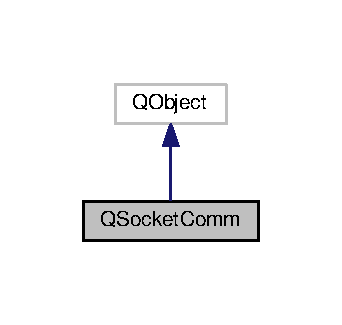
\includegraphics[width=164pt]{class_q_socket_comm__inherit__graph}
\end{center}
\end{figure}


Collaboration diagram for Q\+Socket\+Comm\+:\nopagebreak
\begin{figure}[H]
\begin{center}
\leavevmode
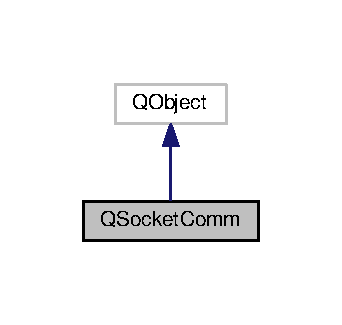
\includegraphics[width=164pt]{class_q_socket_comm__coll__graph}
\end{center}
\end{figure}
\subsection*{Public Member Functions}
\begin{DoxyCompactItemize}
\item 
{\bfseries Q\+Socket\+Comm} (std\+::string host\+\_\+name, uint port\+\_\+number, Q\+Object $\ast$parent=0)\hypertarget{class_q_socket_comm_afe66e31a1196650b60883380ae7dd141}{}\label{class_q_socket_comm_afe66e31a1196650b60883380ae7dd141}

\item 
void {\bfseries Send} (std\+::string command, std\+::string terminator=\char`\"{}\textbackslash{}n\char`\"{})\hypertarget{class_q_socket_comm_a6642ec94f586abdb30dfe0c0532b3bca}{}\label{class_q_socket_comm_a6642ec94f586abdb30dfe0c0532b3bca}

\item 
void {\bfseries Send\+Scl} (std\+::string command)\hypertarget{class_q_socket_comm_a900132260caef9b4e8b959350a5dfd06}{}\label{class_q_socket_comm_a900132260caef9b4e8b959350a5dfd06}

\item 
std\+::string {\bfseries Receive} ()\hypertarget{class_q_socket_comm_af3bd1b626085af405bd27dacf54950e1}{}\label{class_q_socket_comm_af3bd1b626085af405bd27dacf54950e1}

\item 
std\+::string {\bfseries Receive\+Safe} ()\hypertarget{class_q_socket_comm_a7e695332f9bca48a446bf446bd59acda}{}\label{class_q_socket_comm_a7e695332f9bca48a446bf446bd59acda}

\end{DoxyCompactItemize}


The documentation for this class was generated from the following files\+:\begin{DoxyCompactItemize}
\item 
/home/bephillips2/\+Qt-\/\+Projects/\+Electric\+\_\+\+Tiger\+\_\+\+D\+A\+Q/\+Socket\+Communicators/\+Socket\+Comm/q\+\_\+socket\+\_\+comm.\+h\item 
/home/bephillips2/\+Qt-\/\+Projects/\+Electric\+\_\+\+Tiger\+\_\+\+D\+A\+Q/\+Socket\+Communicators/\+Socket\+Comm/q\+\_\+socket\+\_\+comm.\+cpp\end{DoxyCompactItemize}

\hypertarget{class_right_click_menu}{}\section{Right\+Click\+Menu Class Reference}
\label{class_right_click_menu}\index{Right\+Click\+Menu@{Right\+Click\+Menu}}


Inheritance diagram for Right\+Click\+Menu\+:
\nopagebreak
\begin{figure}[H]
\begin{center}
\leavevmode
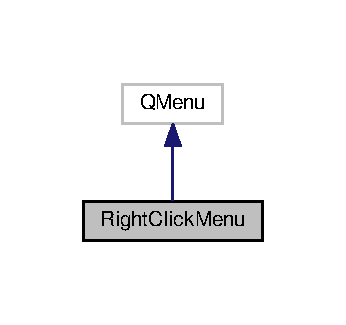
\includegraphics[width=166pt]{class_right_click_menu__inherit__graph}
\end{center}
\end{figure}


Collaboration diagram for Right\+Click\+Menu\+:
\nopagebreak
\begin{figure}[H]
\begin{center}
\leavevmode
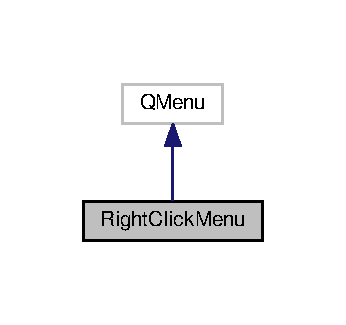
\includegraphics[width=166pt]{class_right_click_menu__coll__graph}
\end{center}
\end{figure}
\subsection*{Signals}
\begin{DoxyCompactItemize}
\item 
void {\bfseries Scaling} ()\hypertarget{class_right_click_menu_a5607dbc6616a76b431cd77ce47d6a1ee}{}\label{class_right_click_menu_a5607dbc6616a76b431cd77ce47d6a1ee}

\end{DoxyCompactItemize}
\subsection*{Public Member Functions}
\begin{DoxyCompactItemize}
\item 
{\bfseries Right\+Click\+Menu} (Q\+Widget $\ast$parent)\hypertarget{class_right_click_menu_afa4f52467f82c6d5de54999ba037428f}{}\label{class_right_click_menu_afa4f52467f82c6d5de54999ba037428f}

\end{DoxyCompactItemize}


The documentation for this class was generated from the following files\+:\begin{DoxyCompactItemize}
\item 
/home/bephillips2/\+Qt-\/\+Projects/\+Electric\+\_\+\+Tiger\+\_\+\+D\+A\+Q/\+Spectrum\+Analyzer/\+Graphic\+Objects/rightclickmenu.\+h\item 
/home/bephillips2/\+Qt-\/\+Projects/\+Electric\+\_\+\+Tiger\+\_\+\+D\+A\+Q/\+Spectrum\+Analyzer/\+Graphic\+Objects/rightclickmenu.\+cpp\end{DoxyCompactItemize}

\hypertarget{class_signal_generator}{}\section{Signal\+Generator Class Reference}
\label{class_signal_generator}\index{Signal\+Generator@{Signal\+Generator}}


Inheritance diagram for Signal\+Generator\+:
\nopagebreak
\begin{figure}[H]
\begin{center}
\leavevmode
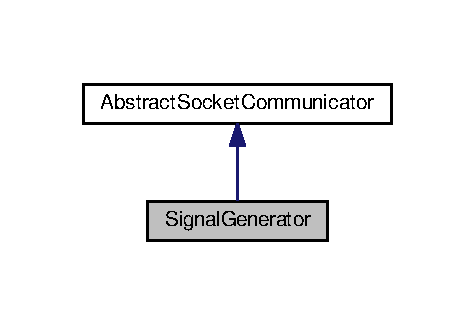
\includegraphics[width=228pt]{class_signal_generator__inherit__graph}
\end{center}
\end{figure}


Collaboration diagram for Signal\+Generator\+:
\nopagebreak
\begin{figure}[H]
\begin{center}
\leavevmode
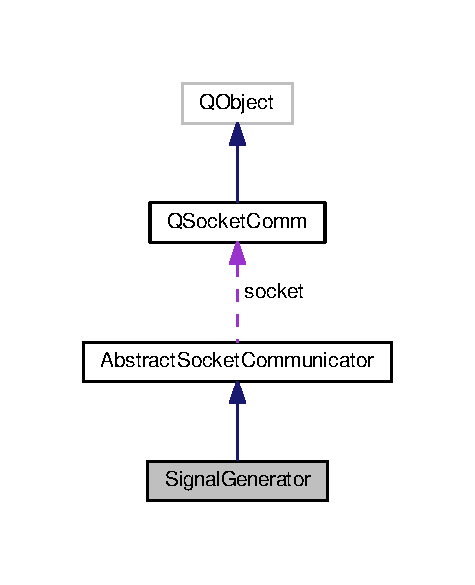
\includegraphics[width=228pt]{class_signal_generator__coll__graph}
\end{center}
\end{figure}
\subsection*{Public Member Functions}
\begin{DoxyCompactItemize}
\item 
{\bfseries Signal\+Generator} (std\+::string ip\+\_\+addr, uint port\+\_\+number)\hypertarget{class_signal_generator_a8e6b4d36b320d50961f83761c5811567}{}\label{class_signal_generator_a8e6b4d36b320d50961f83761c5811567}

\item 
\hyperlink{class_signal_generator}{Signal\+Generator} \& {\bfseries operator=} (const \hyperlink{class_signal_generator}{Signal\+Generator} \&)=delete\hypertarget{class_signal_generator_a4ee427365a76d62d3645f707cf1baf72}{}\label{class_signal_generator_a4ee427365a76d62d3645f707cf1baf72}

\item 
void {\bfseries R\+F\+On} ()\hypertarget{class_signal_generator_a55fbb51b7bd6b3cef69689eb8a63f0f9}{}\label{class_signal_generator_a55fbb51b7bd6b3cef69689eb8a63f0f9}

\item 
void {\bfseries R\+F\+Off} ()\hypertarget{class_signal_generator_a2f277765a848fe7640fae5b3d79c1714}{}\label{class_signal_generator_a2f277765a848fe7640fae5b3d79c1714}

\item 
void {\bfseries Set\+Frequency} (double freq\+\_\+\+M\+Hz)\hypertarget{class_signal_generator_a9ad69641992a00ef027682d5391df8e8}{}\label{class_signal_generator_a9ad69641992a00ef027682d5391df8e8}

\item 
void {\bfseries Set\+Power} (double power\+\_\+d\+Bm)\hypertarget{class_signal_generator_a319e0ca196dd341b1aab276626a729f3}{}\label{class_signal_generator_a319e0ca196dd341b1aab276626a729f3}

\end{DoxyCompactItemize}
\subsection*{Additional Inherited Members}


The documentation for this class was generated from the following files\+:\begin{DoxyCompactItemize}
\item 
/home/bephillips2/\+Qt-\/\+Projects/\+Electric\+\_\+\+Tiger\+\_\+\+D\+A\+Q/\+Socket\+Communicators/\+Signal\+Generator/signal\+\_\+generator.\+h\item 
/home/bephillips2/\+Qt-\/\+Projects/\+Electric\+\_\+\+Tiger\+\_\+\+D\+A\+Q/\+Socket\+Communicators/\+Signal\+Generator/signal\+\_\+generator.\+cpp\end{DoxyCompactItemize}

\hypertarget{class_socket_comm}{\section{Socket\+Comm Class Reference}
\label{class_socket_comm}\index{Socket\+Comm@{Socket\+Comm}}
}
\subsection*{Public Member Functions}
\begin{DoxyCompactItemize}
\item 
\hypertarget{class_socket_comm_a91848bdb00c5e2fa1d83bfabf2e83e23}{{\bfseries Socket\+Comm} (std\+::string host\+\_\+name, uint port\+\_\+number)}\label{class_socket_comm_a91848bdb00c5e2fa1d83bfabf2e83e23}

\item 
\hypertarget{class_socket_comm_ad76f9593ad58c8899878d2b08ac61266}{void {\bfseries Send} (std\+::string command, std\+::string terminator=\char`\"{}\textbackslash{}n\char`\"{})}\label{class_socket_comm_ad76f9593ad58c8899878d2b08ac61266}

\item 
\hypertarget{class_socket_comm_a9cda97b2727f4a47ef5f7d728737521b}{void {\bfseries Send\+Scl} (std\+::string command)}\label{class_socket_comm_a9cda97b2727f4a47ef5f7d728737521b}

\item 
\hypertarget{class_socket_comm_a854e742d1c9f998f7f0981fe3c77c84e}{std\+::string {\bfseries Receive} ()}\label{class_socket_comm_a854e742d1c9f998f7f0981fe3c77c84e}

\item 
\hypertarget{class_socket_comm_a9c09a1bf47807b3465944a5555a61cec}{std\+::string {\bfseries Receive\+Safe} ()}\label{class_socket_comm_a9c09a1bf47807b3465944a5555a61cec}

\end{DoxyCompactItemize}


The documentation for this class was generated from the following files\+:\begin{DoxyCompactItemize}
\item 
/home/admx/\+Qt-\/\+Projects/\+Electric\+\_\+\+Tiger\+\_\+\+D\+A\+Q/\+Socket\+Communicators/\+Socket\+Comm/socketcomm.\+h\item 
/home/admx/\+Qt-\/\+Projects/\+Electric\+\_\+\+Tiger\+\_\+\+D\+A\+Q/\+Socket\+Communicators/\+Socket\+Comm/socketcomm.\+cpp\end{DoxyCompactItemize}

\hypertarget{class_spectrum_analyzer}{\section{Spectrum\+Analyzer Class Reference}
\label{class_spectrum_analyzer}\index{Spectrum\+Analyzer@{Spectrum\+Analyzer}}
}


Inheritance diagram for Spectrum\+Analyzer\+:\nopagebreak
\begin{figure}[H]
\begin{center}
\leavevmode
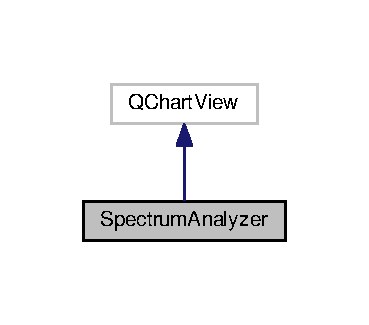
\includegraphics[width=177pt]{class_spectrum_analyzer__inherit__graph}
\end{center}
\end{figure}


Collaboration diagram for Spectrum\+Analyzer\+:\nopagebreak
\begin{figure}[H]
\begin{center}
\leavevmode
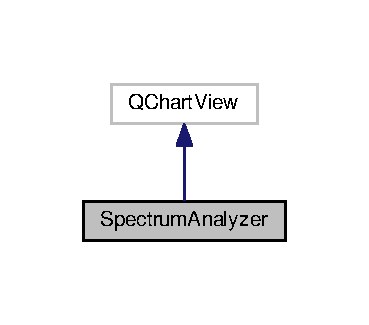
\includegraphics[width=177pt]{class_spectrum_analyzer__coll__graph}
\end{center}
\end{figure}
\subsection*{Public Slots}
\begin{DoxyCompactItemize}
\item 
\hypertarget{class_spectrum_analyzer_aa1979b784bdb752d6f635c4cecb9a4b6}{void {\bfseries Update\+Signal} (std\+::vector$<$ float $>$ time\+\_\+series, uint sample\+\_\+rate)}\label{class_spectrum_analyzer_aa1979b784bdb752d6f635c4cecb9a4b6}

\item 
\hypertarget{class_spectrum_analyzer_a442e34f2e52a974bc33d614c4714a9e3}{void {\bfseries Set\+Frequency\+Min} (double min\+\_\+frequency)}\label{class_spectrum_analyzer_a442e34f2e52a974bc33d614c4714a9e3}

\item 
\hypertarget{class_spectrum_analyzer_aeb522d65cc87a8491f2480b3ec1cf133}{void {\bfseries Set\+Power\+Min} (double min\+\_\+power)}\label{class_spectrum_analyzer_aeb522d65cc87a8491f2480b3ec1cf133}

\item 
\hypertarget{class_spectrum_analyzer_ad1d9bf78ce633b097641ee092645daae}{void {\bfseries Set\+Frequency\+Max} (double max\+\_\+frequency)}\label{class_spectrum_analyzer_ad1d9bf78ce633b097641ee092645daae}

\item 
\hypertarget{class_spectrum_analyzer_adcaf09fb5f0449b6dd95b97e2469af47}{void {\bfseries Set\+Power\+Max} (double max\+\_\+power)}\label{class_spectrum_analyzer_adcaf09fb5f0449b6dd95b97e2469af47}

\item 
\hypertarget{class_spectrum_analyzer_a7edc26864d46ebddd34257ff0d6bc8b7}{void {\bfseries Change\+To\+Volts} ()}\label{class_spectrum_analyzer_a7edc26864d46ebddd34257ff0d6bc8b7}

\item 
\hypertarget{class_spectrum_analyzer_af8f497cd56535515bc17319236fb0524}{void {\bfseries Change\+Tod\+Bm} ()}\label{class_spectrum_analyzer_af8f497cd56535515bc17319236fb0524}

\end{DoxyCompactItemize}
\subsection*{Signals}
\begin{DoxyCompactItemize}
\item 
\hypertarget{class_spectrum_analyzer_afcbb7dc1848df0eb7d43160e489b8855}{void {\bfseries Signal\+Changed} ()}\label{class_spectrum_analyzer_afcbb7dc1848df0eb7d43160e489b8855}

\end{DoxyCompactItemize}
\subsection*{Public Member Functions}
\begin{DoxyCompactItemize}
\item 
\hypertarget{class_spectrum_analyzer_aef258c587abbeb0b11cb765e5aeee636}{{\bfseries Spectrum\+Analyzer} (Q\+Widget $\ast$parent=0)}\label{class_spectrum_analyzer_aef258c587abbeb0b11cb765e5aeee636}

\item 
\hypertarget{class_spectrum_analyzer_ae63398cc69e47a9b3aa463ebbc8ccb1b}{{\footnotesize template$<$class T , typename F $>$ }\\void {\bfseries Plot\+Auto\+Scale} (const T \&y\+\_\+signal\+\_\+elements, F x\+\_\+frequency\+\_\+range)}\label{class_spectrum_analyzer_ae63398cc69e47a9b3aa463ebbc8ccb1b}

\item 
\hypertarget{class_spectrum_analyzer_a102f90cf20b6e157dc9e95d11847c2c1}{{\footnotesize template$<$class T $>$ }\\void {\bfseries Plot} (const T \&y\+\_\+signal\+\_\+elements, double x\+\_\+frequency\+\_\+range)}\label{class_spectrum_analyzer_a102f90cf20b6e157dc9e95d11847c2c1}

\end{DoxyCompactItemize}


The documentation for this class was generated from the following files\+:\begin{DoxyCompactItemize}
\item 
/home/admx/\+Qt-\/\+Projects/\+Electric\+\_\+\+Tiger\+\_\+\+D\+A\+Q/\+Panels/\+Spectrum\+Analyzer/spectrumanalyzer.\+h\item 
/home/admx/\+Qt-\/\+Projects/\+Electric\+\_\+\+Tiger\+\_\+\+D\+A\+Q/\+Panels/\+Spectrum\+Analyzer/spectrumanalyzer.\+cpp\end{DoxyCompactItemize}

\hypertarget{class_stepper_motor}{}\section{Stepper\+Motor Class Reference}
\label{class_stepper_motor}\index{Stepper\+Motor@{Stepper\+Motor}}
\subsection*{Public Member Functions}
\begin{DoxyCompactItemize}
\item 
{\bfseries Stepper\+Motor} (std\+::string ip\+\_\+addr, uint port\+\_\+number)\hypertarget{class_stepper_motor_a60b5baede3214f0774dd4fe166ab6bd5}{}\label{class_stepper_motor_a60b5baede3214f0774dd4fe166ab6bd5}

\item 
\hyperlink{class_stepper_motor}{Stepper\+Motor} \& {\bfseries operator=} (const \hyperlink{class_stepper_motor}{Stepper\+Motor} \&)=delete\hypertarget{class_stepper_motor_aeeceb8eefbcffef0cb0c2b742ffe3603}{}\label{class_stepper_motor_aeeceb8eefbcffef0cb0c2b742ffe3603}

\end{DoxyCompactItemize}


The documentation for this class was generated from the following file\+:\begin{DoxyCompactItemize}
\item 
/home/bephillips2/\+Qt-\/\+Projects/\+Electric\+\_\+\+Tiger\+\_\+\+D\+A\+Q/\+Socket\+Communicators/\+Stepper\+Motor/stepper\+\_\+motor.\+h\end{DoxyCompactItemize}

\hypertarget{class_switch}{\section{Switch Class Reference}
\label{class_switch}\index{Switch@{Switch}}
}


Inheritance diagram for Switch\+:\nopagebreak
\begin{figure}[H]
\begin{center}
\leavevmode
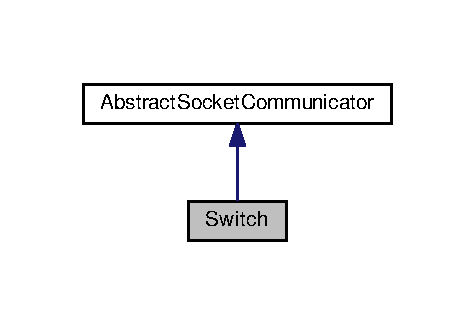
\includegraphics[width=228pt]{class_switch__inherit__graph}
\end{center}
\end{figure}


Collaboration diagram for Switch\+:\nopagebreak
\begin{figure}[H]
\begin{center}
\leavevmode
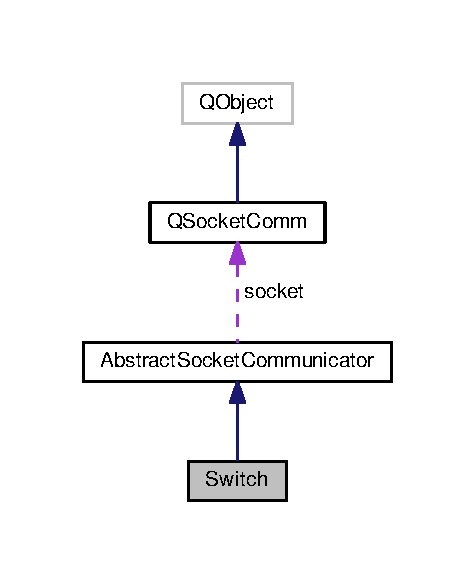
\includegraphics[width=228pt]{class_switch__coll__graph}
\end{center}
\end{figure}
\subsection*{Public Member Functions}
\begin{DoxyCompactItemize}
\item 
\hypertarget{class_switch_a8075f9eb1d911ee97166f9d6c424b766}{{\bfseries Switch} (std\+::string ip\+\_\+addr, uint port\+\_\+number)}\label{class_switch_a8075f9eb1d911ee97166f9d6c424b766}

\item 
\hypertarget{class_switch_a5d75382f2acb13883c3ef60d8b2aef7d}{\hyperlink{class_switch}{Switch} \& {\bfseries operator=} (const \hyperlink{class_switch}{Switch} \&)=delete}\label{class_switch_a5d75382f2acb13883c3ef60d8b2aef7d}

\item 
\hypertarget{class_switch_a88b6be045896b8946be86202dc4c97e3}{void {\bfseries Switch\+To\+Network\+Analyzer} ()}\label{class_switch_a88b6be045896b8946be86202dc4c97e3}

\item 
\hypertarget{class_switch_a004bbaf7459b48549f87f7b26e9353ed}{void {\bfseries Switch\+To\+Digitizer} ()}\label{class_switch_a004bbaf7459b48549f87f7b26e9353ed}

\item 
\hypertarget{class_switch_a9671dbed18c34b5e0e4c8961004d150e}{void {\bfseries Switch\+To\+Transmission} ()}\label{class_switch_a9671dbed18c34b5e0e4c8961004d150e}

\item 
\hypertarget{class_switch_abe4a4b4754fdb4979ddfa3a10fc9e127}{void {\bfseries Switch\+To\+Reflection} ()}\label{class_switch_abe4a4b4754fdb4979ddfa3a10fc9e127}

\end{DoxyCompactItemize}
\subsection*{Additional Inherited Members}


The documentation for this class was generated from the following files\+:\begin{DoxyCompactItemize}
\item 
/home/admx/\+Qt-\/\+Projects/\+Electric\+\_\+\+Tiger\+\_\+\+D\+A\+Q/\+Socket\+Communicators/\+Switch/switch.\+h\item 
/home/admx/\+Qt-\/\+Projects/\+Electric\+\_\+\+Tiger\+\_\+\+D\+A\+Q/\+Socket\+Communicators/\+Switch/switch.\+cpp\end{DoxyCompactItemize}

\hypertarget{struct_volts_tod_bm___f_f_t_correction}{}\section{Volts\+Tod\+Bm\+\_\+\+F\+F\+T\+Correction Struct Reference}
\label{struct_volts_tod_bm___f_f_t_correction}\index{Volts\+Tod\+Bm\+\_\+\+F\+F\+T\+Correction@{Volts\+Tod\+Bm\+\_\+\+F\+F\+T\+Correction}}
\subsection*{Public Member Functions}
\begin{DoxyCompactItemize}
\item 
{\bfseries Volts\+Tod\+Bm\+\_\+\+F\+F\+T\+Correction} (float signal\+\_\+size)\hypertarget{struct_volts_tod_bm___f_f_t_correction_a0a4bc4668c833489861e695f850a77e0}{}\label{struct_volts_tod_bm___f_f_t_correction_a0a4bc4668c833489861e695f850a77e0}

\item 
void {\bfseries operator()} (float \&voltage) const \hypertarget{struct_volts_tod_bm___f_f_t_correction_ae989253eee4929035aefa5c85dc77cac}{}\label{struct_volts_tod_bm___f_f_t_correction_ae989253eee4929035aefa5c85dc77cac}

\end{DoxyCompactItemize}
\subsection*{Public Attributes}
\begin{DoxyCompactItemize}
\item 
float {\bfseries val}\hypertarget{struct_volts_tod_bm___f_f_t_correction_a1e301eb193f2a998e8dafe336d964a8b}{}\label{struct_volts_tod_bm___f_f_t_correction_a1e301eb193f2a998e8dafe336d964a8b}

\end{DoxyCompactItemize}


The documentation for this struct was generated from the following file\+:\begin{DoxyCompactItemize}
\item 
/home/bephillips2/\+Qt-\/\+Projects/\+Electric\+\_\+\+Tiger\+\_\+\+D\+A\+Q/\+Spectrum\+Analyzer/spectrumanalyzer.\+cpp\end{DoxyCompactItemize}

%--- End generated contents ---

% Index
\backmatter
\newpage
\phantomsection
\clearemptydoublepage
\addcontentsline{toc}{chapter}{Index}
\printindex

\end{document}
